\subsection{\label{subsec:FZV1}Brechungsindex und Dispersion}
Aus den Maxwellgleichungen lassen sich für elektromagnetische Wellen in Materie folgende 
Materialgleichungen herleiten, die die Antwort von Materialien auf angelegte Felder beschreiben
\begin{alignat}{2}
    \mathbf{B} &= \mu_{0}\left(\mathbf{H} + \mathbf{M}\right)&&= \mu_{\text{r}}(\omega)\mu_{0}\mathbf{H} \\
    \mathbf{D} &= \epsilon_{0}\mathbf{E} + \mathbf{P} &&= \epsilon_{\text{r}}(\omega)\epsilon_{0}\mathbf{E} \label{eq:lorenz}
\end{alignat}
Hierbei bezeichnen $\mathbf{H}$ die magnetische Feldstärke,
$\mathbf{M}$ die Magnetisierung und 
$\mathbf{B}$ die magnetische Flussdichte, 
sowie $\mathbf{E}$ die elektrische Feldstärke, 
$\mathbf{P}$ die Polarisation 
und $\mathbf{D}$ die elektrische Flussdichte.
$\epsilon_{0}$ und $\mu_{0}$ sind die elektrische und magnetische Feldkonstante, während 
die dielektrische Funktion $\epsilon_{\text{r}}(\omega)$ und die relative Permeabilität $\mu_{\text{r}}(\omega)$
die frequenzabhängige Antwort des Systems beschreiben. 
Aus der allgemeinen Wellengleichung lässt sich die Phasengeschwindigkeit $v_{\text{ph}}$ in Materie 
wie folgt berechnen, woraus die Definition des Brechungsindexes $\tilde{n}$ resultiert 
($c$ beschreibt die Phasengeschwindigkeit im Vakuum, was der Lichtgeschwindigkeit entspricht)
\begin{align}
    \left(\frac{1}{v_{\text{ph}}^{2}}\frac{\partial^{2}}{\partial t^{2}} - \nabla^{2}\right)\mathbf{E} &= 0 \\
    \Rightarrow v_{\text{ph}} &= \frac{c}{\sqrt{\epsilon_{\text{r}}\mu_{\text{r}}}} \coloneqq \frac{c}{\tilde{n}} \\
    \Rightarrow \tilde{n}(\omega) &= \sqrt{\epsilon_{\text{r}}\mu_{\text{r}}}.
\end{align}
Der Brechungsindex ist im Allgemeinfall eine komplexe Größe, für welche wir folgende Notation wählen
\begin{equation}
    \tilde{n} = n + i\kappa.
\end{equation}
Betrachtet man die allgemeine Wellenform des elektrischen Feldes, so ergibt sich 
\begin{align}
    \mathbf{E} &= \mathbf{E}_{0}e^{i\left(\mathbf{k}\cdot\mathbf{r} - \omega t\right)} \\
    &= \mathbf{E}_{0}e^{i\left(\frac{\omega \tilde{n}}{c}\mathbf{e}_{\text{k}}\cdot\mathbf{r} - \omega t\right)} \\
    &= \mathbf{E}_{0}e^{i\left(\frac{\omega n}{c}\mathbf{e}_{\text{k}}\cdot\mathbf{r} - \omega t\right)}e^{-\frac{\omega}{c}\kappa\mathbf{e}_{\text{k}}\cdot\mathbf{r}}, 
\end{align}
was zeigt, dass der Realteil des Brechungsindex für die Dispersion verantwortlich ist und dem Imaginärteil die Absorption zugeschrieben wird. \\
Abbildung \ref{fig:brech} zeigt eine theoretische Näherung des Real- und Imaginärteils des komplexen Brechungsindex.
Die Kurvenform ergibt sich aus dem Lorentzschen Oszillatormodell, welches die dielektrische Funktion mittels Gl.~\eqref{eq:lorenz}
errechnet, woraus für unmagnetische Materialien ($\mu_{\text{r}} \approx 1$) direkt der Brechungsindex folgt. 
\begin{figure}[h!]
    \centering
    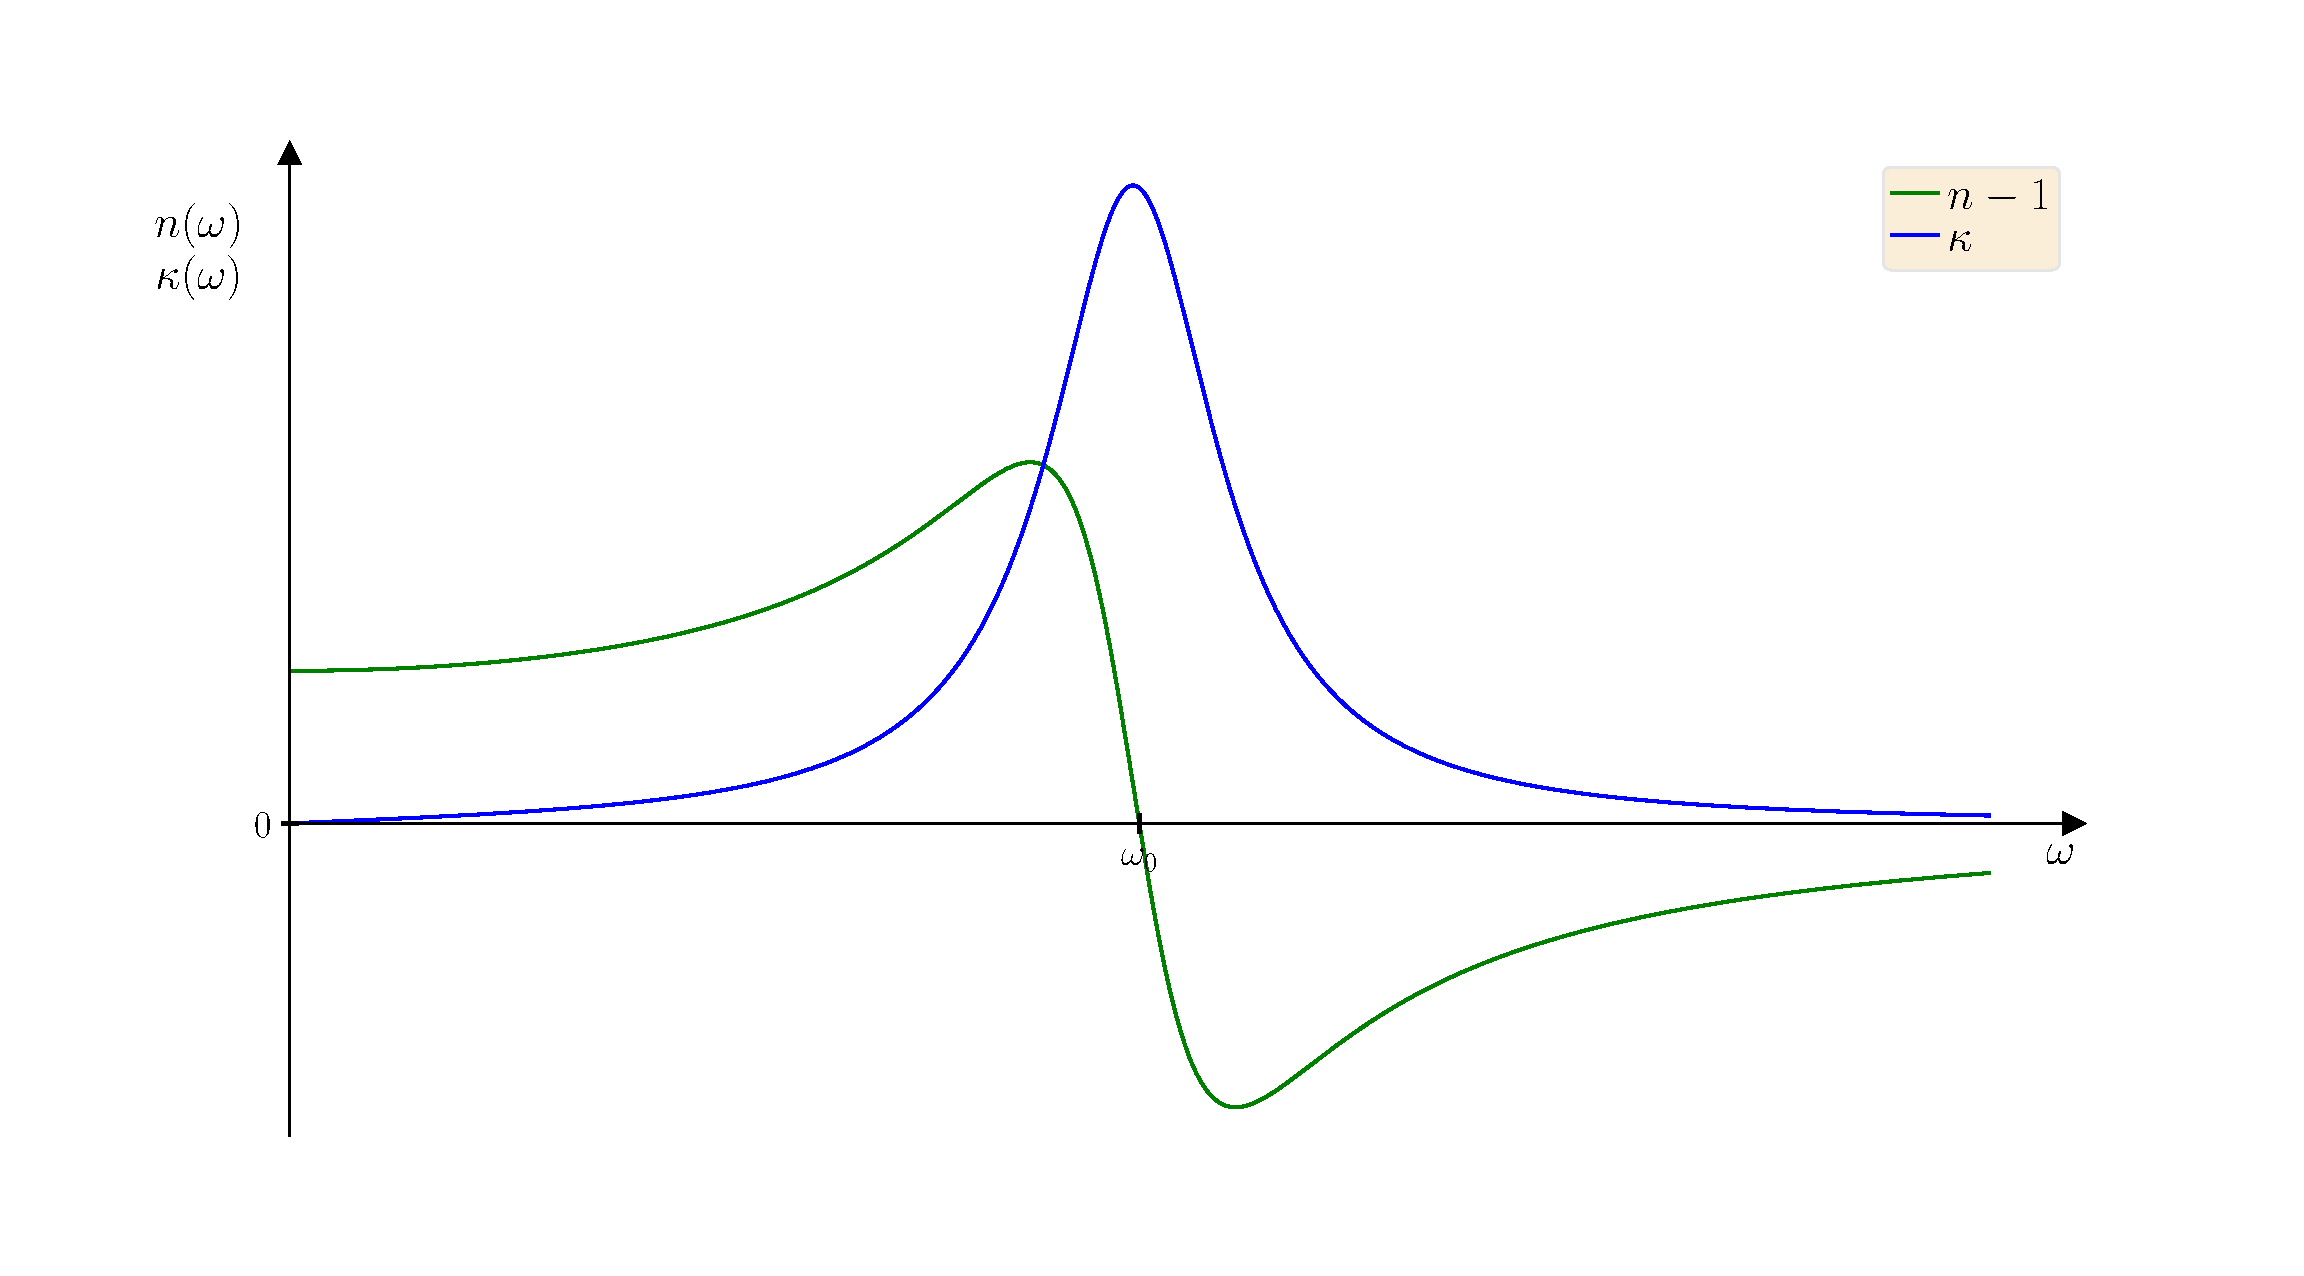
\includegraphics[clip, trim={1cm 1cm 1cm 1cm}, width=0.63\textwidth]{Brech.pdf}
    \caption{\label{fig:brech}Theoretisch errechnete Verläufe des Real- und Imaginärteils des 
    komplexen Brechungsindex als Funktion der Lichtfrequenz $\omega$. Die jeweiligen Funktionen 
    sind um $\omega_{0}$ dargestellt, was der Resonanzfrequenz des Lorentzschen Oszillators entspricht.}
\end{figure}\FloatBarrier\newpage
Außerhalb der Resonanz ist die Ableitung des Realteils nach der Frequenz positiv und die Absorption ist 
sehr gering. Dieser Bereich wird normale 
Dispersion genannt und ist für transparente Medien bei sichtbaren Wellenlängen typisch. 
In der Nähe der Resonanz dreht sich die Steigung des Realteils und geht in die anormale Dispersion 
über. Die Dispersion beschreibt die Veränderung der Phasengeschwindigkeit durch ein Medium als Funktion 
der Frequenz bzw.~der Wellenlänge des Feldes. Es gilt
\begin{align}
    \text{normale Dispersion:}&\hspace{0.5cm}\frac{\text{d}n}{\text{d}\omega} > 0\hspace{0.5cm}\text{bzw.}\hspace{0.5cm}\frac{\text{d}n}{\text{d}\lambda} < 0 \\
    \text{annormale Dispersion:}&\hspace{0.5cm}\frac{\text{d}n}{\text{d}\omega} < 0\hspace{0.5cm}\text{bzw.}\hspace{0.5cm}\frac{\text{d}n}{\text{d}\lambda} > 0 \\
    \frac{\partial v_{\text{ph}}}{\partial \lambda} &= - \frac{c}{n^{2}}\frac{\partial n}{\partial \lambda}.
\end{align}
Für normale Dispersion nimmt die Phasengeschwindigkeit im Medium daher mit steigender Wellenlänge zu, was auch beim Prisma 
beobachtet werden kann, wo blaues kurzwelliges Licht stärker gebrochen wird als rotes langwelliges Licht. \\
Da der Imaginärteil schnell abfällt, wird außerhalb der Resonanz oft $\tilde{n} \approx n$ angenommen [REFS: Gekle, EPC1, Demtröder, Online]. \\